\chapter{Методы поиска информации}
{\bfseries Анонс:}\\\\
Реализация задач конструкционной части. Методы поиска информации в Интернете и оценка ее достоверности.\\\\
{\bfseries Цели:}
\begin{itemize}
	\item{}{\bfseries Обучающие:} Закрепить умения и навыки анализа  технической информации. 
	\item{}{\bfseries Развивающая:} Развить умение извлекать знание из различных источников.\\
\end{itemize}	
{\bfseries Ход занятия:}\\\\
\begin{tabular}[h!]{lll}
	{\hyperlink{lesson26x1}{1. Организационный момент}}&{Презентация}&{(5 мин)}\\
	{\hyperlink{lesson26x2}{2. Конструкционная задача}}&{Практика}&{(15 мин)}\\
	{\hyperlink{lesson26x3}{3. Достоверность информации}}&{Презентация}&{(15 мин)}\\
	{\hyperlink{lesson26x4}{4. Методы поиска информации}}&{Презентация}&{(15 мин)}\\
	{\hyperlink{lesson26x5}{5. Свободное творчество}}&{Практика}&{(60 мин)}\\
	{\hyperlink{lesson26x6}{6. Итоги этапа}}&{Обсуждение}&{(5 мин)}\\
\end{tabular}\\\\

{\hypertarget{lesson26x1}{\blackBlueText{I. Организационный момент}}}\\\\	

В ходе обсуждений новой части конструкционной задачи  в различных командах преподаватель акцентирует внимание учащихся на том, какой информацией они пользуются, можно ли доверять полученной информации, где и как она была получена. Далее проводятся второй и третий разделы данного занятия, посвященные основам работы с информацией, в виде презентацией перед всей группой. В рамках свободного творчества дети решают новую часть конструкционной задачи, используя новые знания по работе с информацией.\\\\

{\hypertarget{lesson26x2}{\blackBlueText{II. Конструкционная задача}}}\\\\

Третья неделя посвящена  другой конструкционной части задачи Автобус механизму открывания дверей. 

Команда должна зафиксировать эту проблему в технической книге и провести коллективное обсуждение путей решения. Могут быть предложены следующие варианты:

\begin{enumerate}
	\item Двери как в новых троллейбусах~--- одностворчатые, поворачивающиеся внутрь.
	\item Двери, как в старых троллейбусах~--- двустворчатые, складывающиеся вовнутрь.
	\item Двери на петлях, открывающиеся внутрь или наружу.
	\item Двери как в метро, раздвигающиеся параллельно сами себе.
\end{enumerate}

Разумеется, нужно опять провести анализ всех высказанных предложений, очертить плюсы и минусы каждого решения. Методы командного обсуждения предполагаются отработанными на предыдущей неделе (Занятие~\ref{lesson25}), поэтому на третьей недели можно обсудить более подробно моменты поиска информации, достоверности источников информации и создание моделей и прототипов отдельных узлов робота.\\\\

{\hypertarget{lesson26x3}{\blackBlueText{III. Достоверность информации}}}\\\\	

Работа над техническим проектом требует непрерывной работы с информацией. Поиск уже имеющихся технических решений, сравнение их друг с другом, мнения, модели, испытания. Поэтому  на данном этапе хочется обсудить с детьми два важнейших вопроса: «Где искать информацию?» и «Как искать информацию?».

Как где? В интернете, конечно! И понятно как, Яндекс, Гугл, к вашим услугам. Так решает для себя эти вопросы современный ребенок. Умеет ли он после этого работать с информацией? Не факт. На практике очень часто приходится сталкиваться с тем, что не найдя искомую информацию по первому запросу, ребенку даже не приходит в голову переформулировать запрос. Дети не понимают принципы работы поисковых машин. Не  оценивают достоверность источников информации.

Итак, все-таки «где?». Нет, не обязательно и даже странно в наше время бежать в библиотеку или лезть в энциклопедию. Но надо понимать, что интернет – это не Большой Всепланетный Информаторий. Это способ получить доступ к тем же энциклопедиям, библиотекам, журналам, газетам, только в электронном виде. Все те же самые, знакомые человеку тысячелетиями источники информации. Какие же из них наиболее надежны? Перечислим их по мере убывания степени достоверности. 

Учебник, энциклопедия, база данных, толковый словарь. Здесь наиболее проверенные, устоявшиеся, тщательно отредактированные знания. «Ляпы» встречаются, но крайне редко.

Оригинальная статья, обзор, специальная монография.  Основные источники научной информации с системой перекрестных ссылок. Основные ошибки связаны с погрешностями и ошибками экспериментов, не видных редакторам и рецензентам, новые непроверенные концепции. 

Научно-популярный, познавательный журнал или книга. Цель такого рода изданий – заинтересовать обычного читателя, не владеющего специальными научными языками, побудить его к самостоятельному поиску знаний. Ошибки и неточности возникают из-за потери строгости в процессе упрощения формулировок и теорий для широкого слушателя.

Средства массовой информации (СМИ). Телевидение, газеты, радио~--- это  по большей части всего лишь эффективный способ формирования общественного мнения. В них встречается сознательная ложь, ради пиара и ложь по необразованности журналистов. 

Форумы.  Очень сильно зависит от конкретного форума и уровня его посетителей. Очень часто встречаются откровенные ошибки и просто мнения, но с другой стороны иногда это единственный шанс найти какую-то специфическую, практическую информацию. 

Видно, что в принципе можно использовать информацию из всех вышеперечисленных источников, но желательно, что бы основные факты, на которые опирается ученик, базировались на энциклопедических знаниях, а прочие ресурсы лишь дополняли картину.

Отдельно хочется сказать два слова про Википедию, как наиболее популярный источник информации у детей. Относить ее к энциклопедиям конечно не правильно, т.к. информация в ней не проходила такого жесткого контроля, во многих статьях встречаются ошибки. По степени достоверности ее можно поместить где-то между СМИ и форумами.\\\\

{\hypertarget{lesson26x4}{\blackBlueText{IV. Методы поиска информации}}}\\\\

Итак, как относиться к найденной информации, в зависимости от ее источника понятно. Остался вопрос как ее найти. Главным способом поиска, разумеется являются поисковые машины. Наиболее распространенное заблуждение состоит в том, что  поисковые машины ищут информацию по всей сети Internet. На самом деле это не совсем верно. Если бы при реализации алгоритма работы поисковых машин был использован такой подход, то для обработки только одного запроса и выдачи результатов потребовалось бы несколько дней. Поэтому, практически реализована иная схема работы поисковой машины. Каждая поисковая машина имеет и постоянно пополняет свою ({\bfseries локальную}) базу данных. База данных поисковой машины содержит основные параметры ({\bfseries индексы}) каждого известного данной машине (проиндексированного) документа. Каждая поисковая машина использует свои методы индексации. Кроме того, различные поисковые машины имеют разные объемы базы данных.\\\\

В результате, механизм обработки запроса пользователя поисковой машиной выглядит следующим образом:

\begin{itemize}
	\item в соответствии с заданным в запросе ключевым словом или словосочетанием, машина проводит поиск в своей локальной базе данных, сверяя ключевое слово с наборами ключевых слов, соответствующих каждому документу из её базы данных;
	\item затем, используя соответствующие алгоритмы, поисковая машина сортирует результаты поиска и выдает их пользователю;
	\item в результате сортировки результатов, в начало списка помещаются наиболее соответствующие (с точки зрения поисковой машины) ключевым словам документы.
\end{itemize}

В связи с огромным количеством информации, размещенной в сети, ни одна из поисковых машин не в состоянии просмотреть все документы. Каждая поисковая машина индексирует только часть их. Все остальные документы, а к сожалению это большая часть ресурсов, найти с ее помощью не удастся.

Отсюда очевидным образом вытекает, что если ваш поиск закончился неудачей, это не значит, что нужной информации в сети нет. Кроме того, очень важно научиться грамотно формулировать запрос поисковой машине.\\\\

Некоторые практические рекомендации по поиску информации можно свести к следующим:

\begin{itemize}
	\item Формируйте поисковый запрос из нескольких ключевых слов, определяющих тему, однако помните,  что если вы вводите запрос к поисковой машине, состоящий из нескольких слов, то в результате получаете список документов, в которых встречается хотя бы одно слово.
	\item Не бойтесь менять поисковые запросы много раз за поиск.
	\item Ищите информацию несколькими разными поисковыми машинами.
	\item Не задавайте вопросы, пишите начала возможных ответов.
	\item Для поиска редкой информации попробуйте сначала найти общие ресурсы по теме, на них могут быть ссылки уже на специальные ресурсы.
	\item Для поиска документа с точной цитатой возьмите поисковый запрос в кавычки.
	\item Указывайте слова, которые не должны встречаться в искомых документах. Обычно для этого используют либо знак ''--'', либо ключевое слово NOT.\\\\
\end{itemize}

{\hypertarget{lesson26x5}{\blackBlueText{V. Свободное творчество}}}\\\\

Для команд, опережающих своих товарищей, на этом этапе можно ввести элемент более глубокого анализа.  Это позволит им поработать на чуть более серьезном уровне, оставаясь в рамках той же темы, а другим командам догнать их. 

Предлагается рассмотреть возможные технические решения не только теоретическим образом, обсудив найденную по каждому варианту информацию, но и создать работающую модель каждого узла и на практике проверить все плюсы и минусы каждого решения. Получив такое дополнительное задание от преподавателя команда должна закрепить каждую модель за конкретным участником, договориться о формате доклада по модели, создать работающие прототипы узлов (открывания дверей, в данном примере) и провести итоговое обсуждение вариантов. Разумеется, на каждом этапе необходимо наблюдение и помощь преподавателя.\\\\

{\hypertarget{lesson26x6}{\blackBlueText{IV. Итоги этапа}}}\\\\	

Общие результаты четвертого этапа, вне зависимости от конкретной задачи, должны выглядеть так:

\begin{itemize}
	\item Сформулированы  проблемы конструкционной части.
	\item Рассмотрены различные пути решения проблем. Проведено обсуждение плюсов и минусов различных вариантов.
	\item Решены практически все проблемы конструкционной части.
	\item Отлажена система командного взаимодействия.
	\item Успешно реализуются принципы написания технической книги.
\end{itemize}

Рассмотрим, для примера, записи, сделанные по итогам третьей недели в технической книге проектной группы Автобус ФМЛ № 30 ({\slshape курсивом выделены ремарки автора}): 

{\slshape Нарисован чертеж принципиальной схемы конструкции. Чертеж выполнен понятно, но отсутствуют какие-либо пояснения к нему.
	
	\begin{figure}[h!]
		\begin{center}
			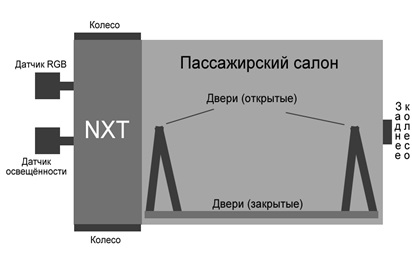
\includegraphics[width=1\linewidth]{chapters/chapter26/images/1}
			\caption{Модель автобуса. Вид сверху.}
			\label{ris:image26x1}
		\end{center}
	\end{figure}
	
	Указано итоговое решение для механизма открывания-закрывания дверей и довольно наглядно описан механизм их работы, но нет следов обсуждения различных вариантов, их недостатков и достоинств, причин выбора итогового варианта.}

В роботе использована конструкция дверей настоящих автобусов. В открытом состоянии они выглядят как на рисунках ниже.

\begin{figure}[h!]
	\begin{center}
		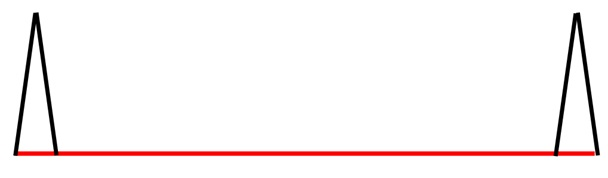
\includegraphics[width=0.9\linewidth]{chapters/chapter26/images/2}
		\caption{Открытые двери. Вид сверху.}
		\label{ris:image26x2}
	\end{center}
\end{figure}


\begin{figure}[h!]
	\begin{center}
		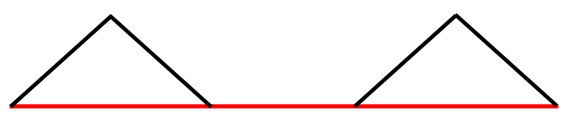
\includegraphics[width=0.88\linewidth]{chapters/chapter26/images/3}
		\caption{Полуоткрытые двери. Вид сверху.}
		\label{ris:image26x3}
	\end{center}
\end{figure}

\begin{figure}[h!]
	\begin{center}
		
\includegraphics[width=0.88\linewidth]{chapters/chapter26/images/4}
		\caption{Закрытые двери. Вид сверху.}
		\label{ris:image26x4}
	\end{center}
\end{figure}	

Поскольку ресурсы ограничены одним набором Lego NXT, Для передачи вращения на вторую дверь используется цепь шестерёнок, которая также меняет направление вращения.

\begin{figure}[h!]
	\begin{center}
		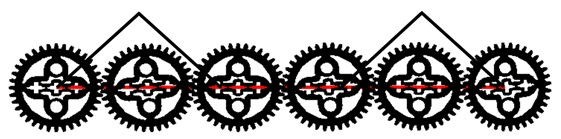
\includegraphics[width=0.88\linewidth]{chapters/chapter26/images/5}
		\caption{Двери с шестерёнками. Вид сверху.}
		\label{ris:image26x5}
	\end{center}
\end{figure}	

\begin{figure}[h!]
	\begin{center}
		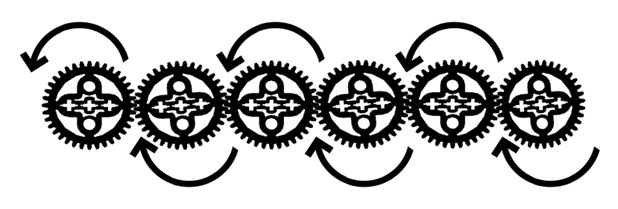
\includegraphics[width=0.88\linewidth]{chapters/chapter26/images/6}
		\caption{Направление движения шестерёнок}
		\label{ris:image26x6}
	\end{center}
\end{figure}